\documentclass[%
 reprint,
 amsmath,amssymb,
 aps,
]{revtex4-1}

\usepackage{graphicx}% Include figure files
\usepackage{dcolumn}% Align table columns on decimal point
\usepackage{bm}% bold math
\usepackage[dvipdfm,colorlinks=true,linkcolor=blue,filecolor=blue, urlcolor=blue]{hyperref}
\usepackage{braket}
\usepackage{caption} % for captionsetup[figure]
\usepackage{threeparttable} % for table caption modification
\usepackage{breqn} % dmath: automatic equation line breaking
\numberwithin{equation}{section}% (p.37)

% \sloppy sets all text to loose spacing, allowing overflow and uneven word spacing;
% not recommended for academic papers requiring strict typesetting.
\tolerance=1000
\emergencystretch=1em
\hyphenpenalty=3000
\exhyphenpenalty=3000
\flushbottom
\usepackage[final]{microtype}

\usepackage{ragged2e}  % for \justifying command
\usepackage{booktabs}


\begin{document}

    \captionsetup[figure]{justification=raggedright,
        labelfont={bf},name={Fig.},labelsep=period} % raggedright for left-aligned figure captions
    \captionsetup[table]{
        labelfont={bf},name={Table.},labelsep=period}


\title{Spin as a Real Vector from Internal Photon-Sphere Motion:\\ Geometric Origin of U(1) Gauge and SU(2) Periodicity}
\author{Satoshi Hanamura}
\email{hana.tensor@gmail.com}
\date{June 15, 2025}



\begin{abstract}
We propose a geometric and deterministic model of electron spin in which spin angular momentum arises from internal reciprocating motion of a confined photon-sphere, rather than from an abstract pseudovector. In this model, spin is described as a real, time-evolving vector whose $z$-component varies as $\sin(2\omega t)$, leading naturally to the $4\pi$ periodicity characteristic of spin-$\frac{1}{2}$ particles. The model corrects a previous dimensional inconsistency by introducing an explicit angular velocity vector $\boldsymbol{\Omega}(t) = -\frac{1}{4c^2} \sin(2\omega t)\,\mathbf{e}_z$, inspired by a reinterpretation of Thomas precession as a physically real effect of internal dynamics.

Spin quantization is interpreted not as the result of probabilistic wavefunction collapse, but as the projection of a continuously oscillating internal state governed by internal time phase. This framework accounts for spin measurements, the anomalous $g$-factor, and Zeeman-like effects without invoking external fields or intrinsic quantum randomness. Instead, these phenomena are explained as relativistic consequences of internal oscillatory motion.

More fundamentally, the model shows that the SU(2) symmetry of spin emerges as a geometric unfolding of an underlying U(1) phase structure. This challenges the standard interpretation of SU(2)$\times$U(1) as a product of independent gauge groups and suggests that apparent features such as parity violation in weak interactions may result from projection artifacts of a symmetric internal geometry. The reinterpretation of spin as a real vector also undermines its classification as a pseudovector, offering a concrete physical basis for the observed $720^\circ$ spinor transformation without relying on abstract group-theoretic axioms. This geometric formulation offers a unified picture of spin, internal phase evolution, and gauge symmetry, bridging quantum and classical frameworks through the deterministic dynamics of internal time.
\end{abstract}


\maketitle

% ========================================
% Section 1: Introduction
% ========================================
\section{Introduction}

This work proposes a geometric reinterpretation of electron spin as a real, time-evolving internal vector, replacing the conventional notion of spin as an abstract pseudovector with probabilistic interpretation~\cite{uhlenbeck1925}. Within this framework, spin emerges from the oscillatory motion of a confined photon-sphere, whose internal time phase governs the energy distribution and angular dynamics of the particle.

Conventional quantum mechanics treats spin as an intrinsic degree of freedom described by SU(2) generators and postulates spin quantization as a fundamental property. The spin vector is modeled as a pseudovector, and its measurement outcomes are probabilistically determined via projection onto eigenstates. However, this description lacks a geometric origin and provides no physical mechanism for the 720-degree periodicity of spin-$\frac{1}{2}$ systems.

The present model addresses these issues by introducing a real-valued internal motion with a well-defined time phase $\omega t$. The spin arises from a sinusoidal angular velocity $\Omega(t) = -\frac{1}{4c^2} \sin(2\omega t) \, \mathbf{e}_z$, which captures the $4\pi$ periodicity of spin states and leads to a deterministic energy distribution at each phase angle. This internal structure eliminates the need for probabilistic collapse and offers an alternative to the Copenhagen interpretation.

Furthermore, this geometric foundation reveals that the SU(2) symmetry governing spin can be reinterpreted as a geometric unfolding of an underlying U(1) phase structure. This suggests that SU(2) and U(1) may not be independent gauge groups but rather projections of a single internal geometric space. In this view, even the parity violation typically associated with SU(2) weak interactions may be reconsidered as an artifact of projection rather than a fundamental asymmetry.

The concept of Zitterbewegung was first introduced by Schrödinger in 1930 \cite{schrodinger1930} as a rapid oscillatory motion predicted by the Dirac equation, where electrons appear to move in circular trajectories at the speed of light. While initially regarded as a mathematical artifact, subsequent work by Barut and Bracken \cite{barut1981} demonstrated that Zitterbewegung could be interpreted as arising from the internal geometry of the electron, suggesting a physical foundation for this phenomenon. Hestenes further developed this interpretation \cite{hestenes1990}, proposing that Zitterbewegung provides a physical basis for spin and magnetic moment through geometric algebra formalism.

Recent experimental advances have provided support for the physical reality of Zitterbewegung-like phenomena. Gerritsma et al. \cite{gerritsma2010} successfully simulated the Dirac equation and its associated trembling motion using trapped ions, while analogous oscillatory dynamics have been observed in photonic systems \cite{zhang2023}. These developments suggest that internal oscillatory structures, rather than being purely theoretical constructs, may have observable physical manifestations.

This paper presents a unified description of spin, internal motion, and gauge symmetry grounded in physical geometry. Section~\ref{sec:motivation} presents the motivation and background for reinterpreting spin as a real vector. Section~\ref{sec:notation} defines the physical quantities and notation used throughout the paper. Section~\ref{sec:discussion} discusses the corrected dimensional formulation, the emergence of angular velocity and its connection to spin and Thomas precession~\cite{thomas1926}, and examines the SU(2) × U(1) gauge structure from a geometric perspective. Section~\ref{sec:conclusion} compares the model with conventional theory and outlines implications for future developments.


% ========================================
% Section 2: Motivation
% ========================================
\section{Motivation}
\label{sec:motivation}

In our earlier formulation of spin dynamics \cite{hanamura2309.0047}, the angular velocity vector $\boldsymbol{\Omega}$ of the internal motion lacked an explicit directional basis, resulting in an inconsistency where a vector was equated to a scalar function. In this paper, we correct this by introducing the $z$-axis unit vector ${\bf e}_z$, revealing that the spin angular velocity oscillates sinusoidally between positive and negative directions. This time-periodic behavior suggests that spin is not fixed prior to measurement, but dynamically varies with internal phase, offering a geometrically grounded picture of spin as a real vector rather than an abstract quantum label.

The question ``What is spin?'' has been a subject of ongoing debate since the early days of quantum mechanics \cite{ohanian1986}. While conventional quantum theory treats spin as an abstract pseudovector with no classical analog, alternative approaches have sought to provide physical interpretations. Baylis \cite{baylis1992} proposed a classical eigenspinor formalism using Clifford algebra, while Hestenes \cite{hestenes1990} suggested that spin emerges from Zitterbewegung as a manifestation of internal rotational dynamics. These approaches share a common goal: to ground quantum spin in physical geometry rather than abstract mathematical formalism.

In contrast to traditional interpretations, our 0-Sphere model interprets spin angular momentum as arising from an internal oscillator whose periodicity leads to the observed 720-degree rotation symmetry of spin-$\frac{1}{2}$ particles. As we problematized in \cite{hanamura2309.0047}, \textbf{this challenges the traditional view that spin results from circular motion with a fixed orientation.} Instead, we show that even reciprocating internal motion can generate angular momentum, implying a geometric origin of the SU(2) symmetry group from an underlying U(1) phase evolution. The measured spin states $\pm 1/2$ emerge as projections onto the $z$-axis of a continuously rotating vector, rather than from discrete eigenstates of an abstract Hilbert space.

% ========================================
% Section 3: Notation and Physical Quantities
% ========================================
\section{Notation and Physical Quantities}
\label{sec:notation}

The following symbols and definitions are used throughout this paper:

\begin{itemize}
    \item $\omega$ : Angular frequency of internal oscillation of the photon-sphere. 
    
    \item $t$ : Proper time parameter within the rest frame of the particle. Governs internal phase evolution.
    
    \item $E_0$ : Rest energy of the electron. Used as the normalization constant in internal energy decomposition.
    
    \item $v(t)$ : Instantaneous internal velocity of the photon-sphere. Typically expressed as $v(t) = \cos(\omega t)$.
    
    \item $a(t)$ : Instantaneous internal acceleration. Typically given as $a(t) = -\sin(\omega t)$.
    
    \item $\boldsymbol{\Omega}(t)$ : Time-dependent internal angular velocity vector. Defined as $\boldsymbol{\Omega}(t) = -\frac{1}{4c^2} \sin(2\omega t) \cdot \mathbf{e}_z$ in natural units.
    
    \item $\mathbf{e}_z$ : Unit vector in the internal $z$-direction, assumed to be the axis of angular precession in the internal geometry.
    
    \item $\cos^4(\omega t/2), \sin^4(\omega t/2)$ : Energy weight functions corresponding to kernel $A$ and kernel $B$ in the internal structure~\cite{hanamura2411.0117}.
    
    \item $\frac{1}{2} \sin^2(\omega t)$ : Kinetic energy contribution of the oscillating photon-sphere at internal time $t$~\cite{hanamura2411.0117}.
    
    \item Kernel $A$, Kernel $B$ : Two complementary internal energy configurations representing oscillatory modes of the confined photon-sphere~\cite{hanamura2411.0117}.
    
    \item $c$ : Speed of light in vacuum. Used explicitly in $\boldsymbol{\Omega}(t)$ to restore dimensions in non-natural units.
\end{itemize}

% ----------------------------------------
% Figure 1: f-double_frequency.png -- Internal motion components
% ----------------------------------------
\begin{figure*}[t!]
    \centering 
    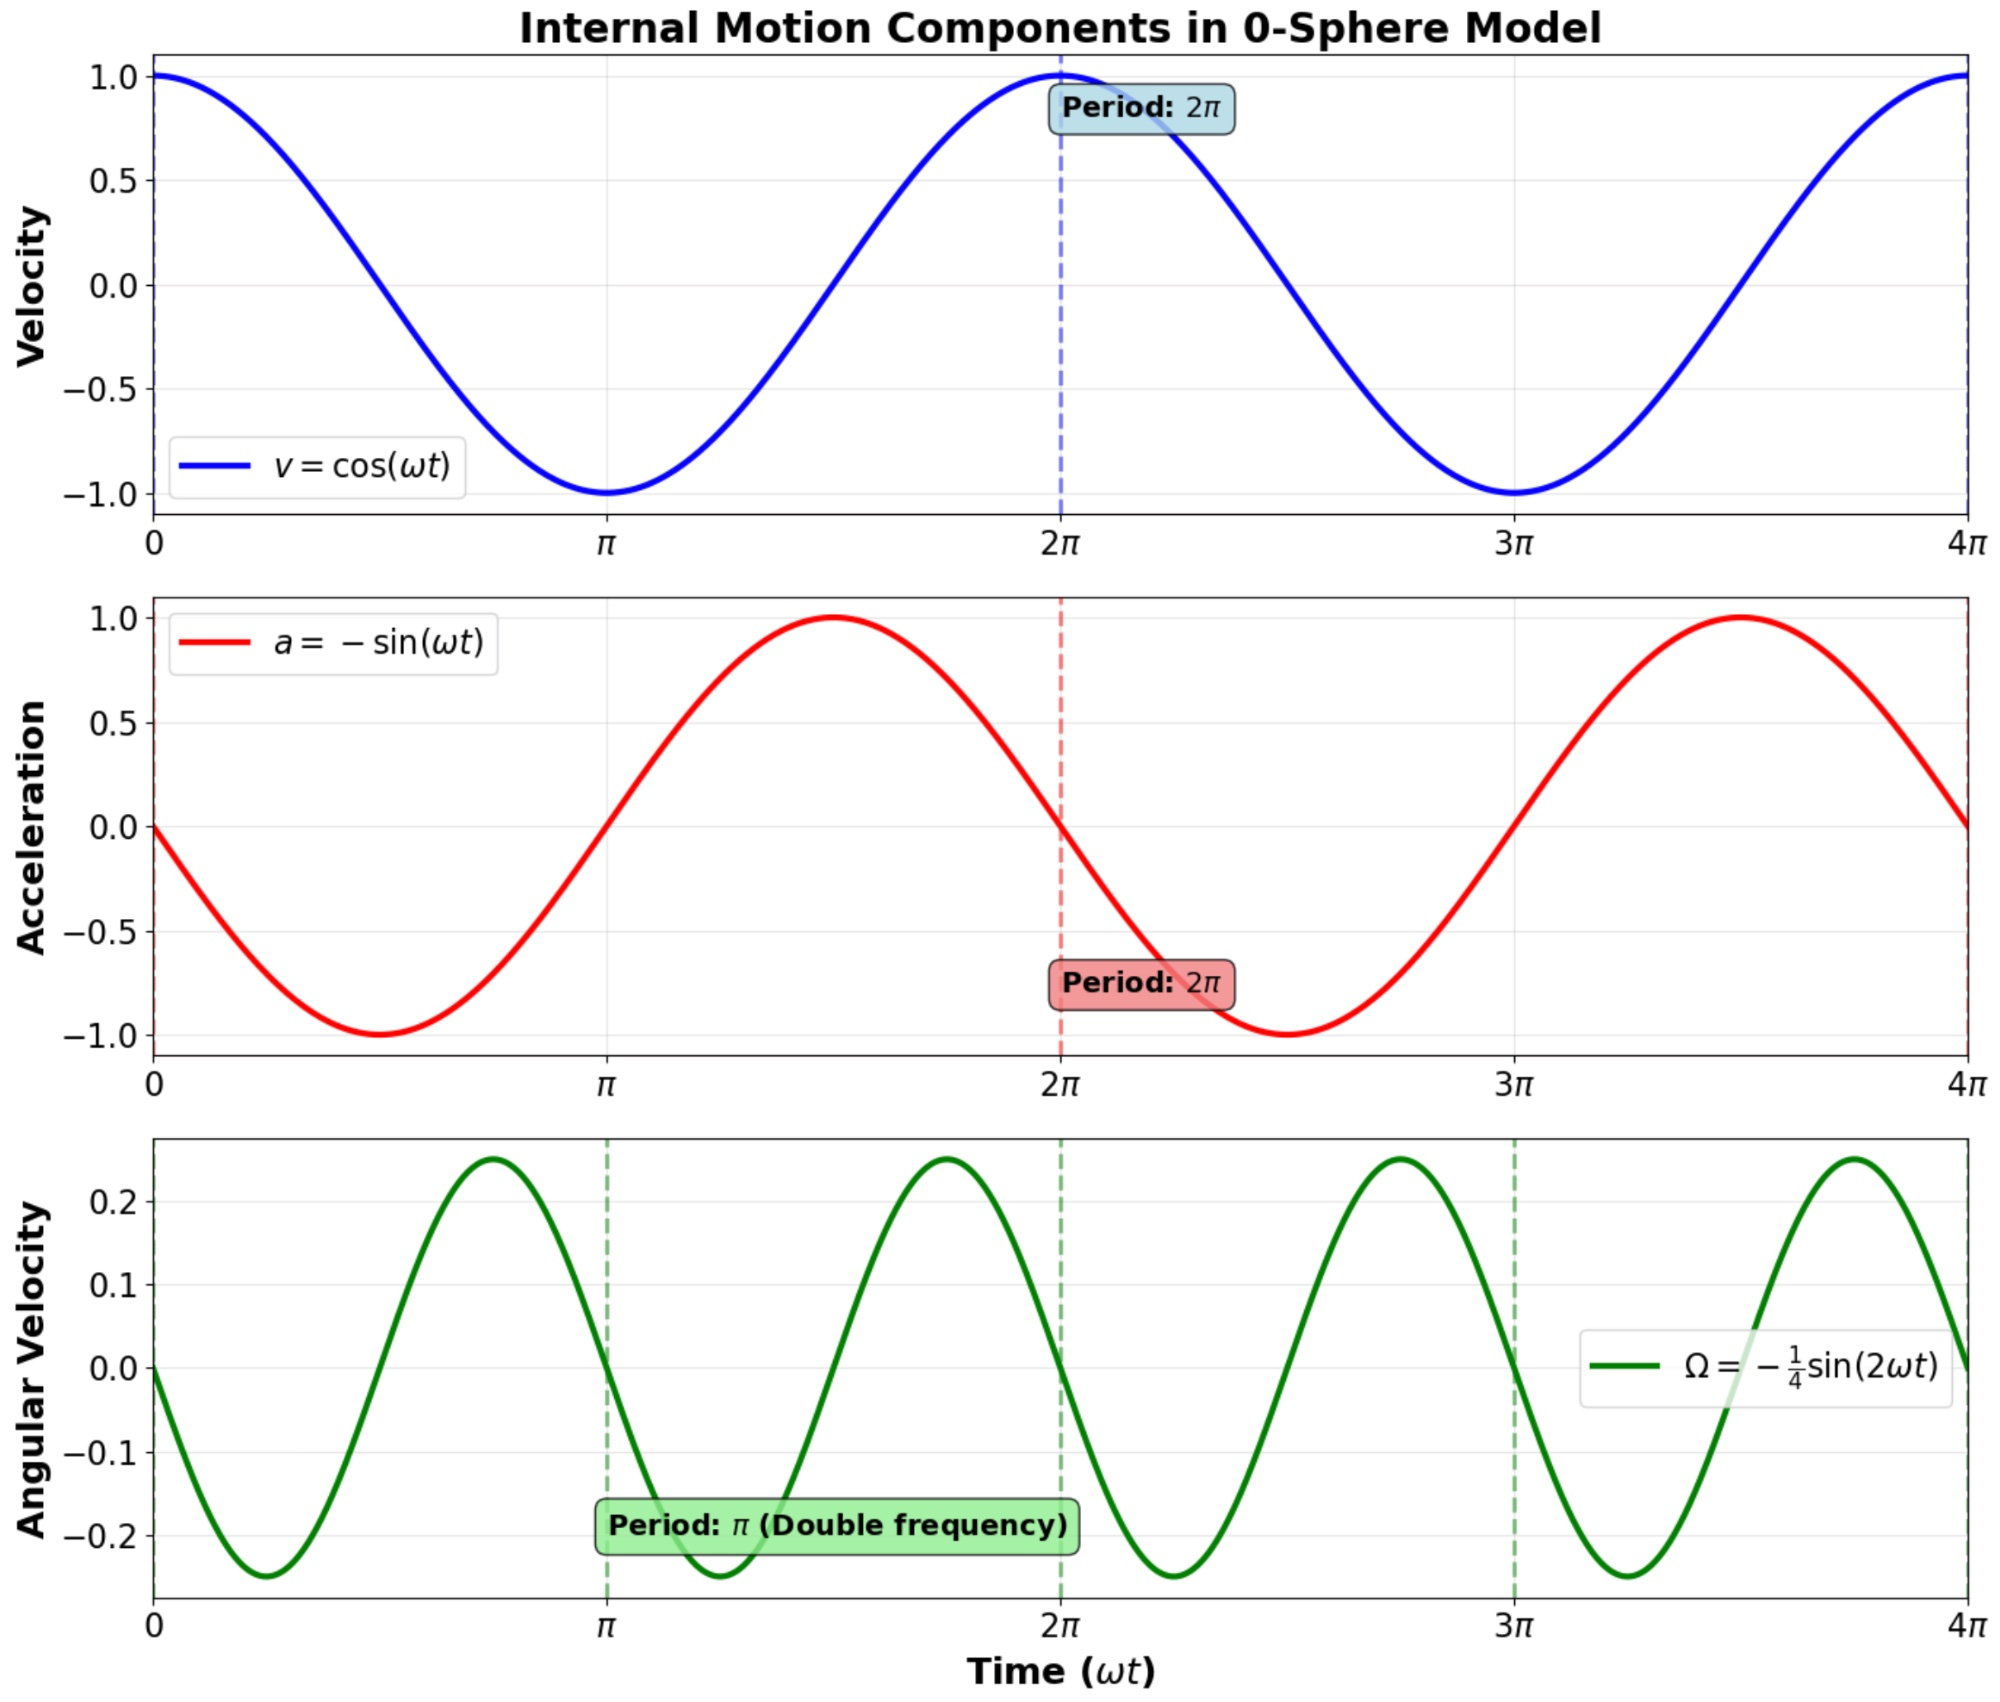
\includegraphics[width=\textwidth]{f-double_frequency.png}
    \caption{\justifying Time evolution of internal motion components in the 0-sphere model. The velocity $v = \cos(\omega t)$ and acceleration $a = -\sin(\omega t)$ each exhibit a period of $2\pi$, while their cross product yields the angular velocity $\Omega(t) = -\frac{1}{4} \sin(2\omega t)$, which exhibits a period of $\pi$. This angular velocity represents the internal precessional dynamics of the spin vector and reveals a frequency doubling relative to the underlying oscillations. This double-frequency behavior leads to a $4\pi$ periodicity in the spin state, providing a geometric origin for the characteristic 720-degree spinor transformation of spin-$\frac{1}{2}$ particles.}
\label{fig:double_frequency}
\end{figure*}


% ========================================
% Section 4: Discussion
% ========================================
\section{Discussion}
\label{sec:discussion}

% ----------------------------------------
% Subsection 4.1: Geometric Emergence of SU(2) from U(1) Phase Evolution
% ----------------------------------------
\subsection{Geometric Emergence of SU(2) from U(1) Phase Evolution}

The 0-Sphere model suggests that the SU(2) symmetry group characterizing spin-$\frac{1}{2}$ systems may emerge from a U(1)-type internal phase rotation. The internal oscillator of the photon-sphere exhibits $2\pi$ periodicity in phase but $4\pi$ periodicity in the observable angular momentum. This phase-doubling relationship directly reflects the spinor property of requiring a $4\pi$ rotation to return to the original quantum state.

This frequency doubling is explicitly demonstrated in Fig.~\ref{fig:double_frequency}, where the velocity and acceleration components oscillate with period $2\pi$, while their cross product—which generates angular momentum—oscillates with period $\pi$, corresponding to twice the fundamental frequency.

This phenomenon is typically introduced axiomatically in quantum mechanics via two-component spinors. However, in our model, it arises from the real-valued structure of vector cross products and phase reversal. The geometric foundation for this interpretation was laid by Hestenes \cite{hestenes1990}, who showed that the complex phase factor in the Dirac wave function admits a physical interpretation through Zitterbewegung. In his formulation, the unit imaginary $i$ in quantum mechanics corresponds to a generator of spacetime rotations.

In our model, the vector components of velocity, acceleration, and angular velocity map one-to-one onto the internal temporal phase via real-valued vector operations and phase inversion. This makes the emergence of SU(2) symmetry from U(1) phase evolution a direct geometric consequence, rather than an abstract mathematical postulate.

The notion that spin arises from internal oscillatory motion is not new. Hestenes demonstrated that the Dirac equation inherently describes a helical motion—Zitterbewegung—that encodes both spin and magnetic moment as geometric features of a rapidly rotating internal structure \cite{hestenes2010}.

In our formulation, this internal motion traces a closed trajectory on a 0-sphere, with a well-defined phase in internal time. The SU(2) symmetry thus appears not as a fundamental gauge symmetry, but as a geometric extension of the underlying U(1) phase associated with internal dynamics. This perspective aligns the abstract algebraic structure of spin with a concrete geometric origin.

In this view, the commonly accepted SU(2) symmetry is not an imposed mathematical requirement but a natural geometric extension of the deeper U(1) phase structure. The quantization of spin can be interpreted as the projection of a deterministic, oscillating vector field onto a measurement axis, with probabilistic outcomes arising from phase-dependent projections rather than intrinsic indeterminacy.

This reinterpretation also casts new light on the conventional classification of spin as a pseudovector. In standard quantum theory, spin is treated as an axial vector—remaining unchanged under spatial inversion—based on group-theoretic transformation properties. However, this classification arises not from experimental observation but from abstract mathematical conventions. Our model suggests a more fundamental geometric explanation: \textbf{this internal spin vector remains unchanged under spatial inversion not because it is an axial vector, but because it arises from a closed U(1) phase space that is geometrically invariant under mirror operations.}

These findings suggest that what is often attributed to fundamental gauge symmetry may instead arise from internal geometric structure, a possibility we further consider in the final summary.


% ----------------------------------------
% Subsection 4.2: Correcting Dimensional Inconsistency in the Angular Velocity
% ----------------------------------------
\subsection{Correcting Dimensional Inconsistency in the Angular Velocity}

Zitterbewegung has often been regarded as a mathematical artifact of the Dirac equation, but recent experiments have directly observed its signatures in both Bose–Einstein condensates and photonic systems. For instance, LeBlanc et al. demonstrated clear detection of position and velocity oscillations in a spin–orbit coupled Bose–Einstein condensate, showing that the amplitude and frequency of Zitterbewegung can be controlled experimentally \cite{leblanc2013}. Specifically, they showed that the amplitude could be tuned by preparing the initial spin state, while the frequency could be adjusted via the strength of the Raman coupling.

Furthermore, Zhang et al. observed lateral oscillations of polariton wave packets in semiconductor microcavities, revealing a photonic analogue of relativistic spin–orbit coupling and the physical reality of Zitterbewegung \cite{zhang2023}. These results not only confirm that Zitterbewegung is an observable phenomenon, but also support the physical plausibility of internal degrees of freedom based on Zitterbewegung-like oscillations, such as those proposed in this work. These observations thus support the foundational assumption of the 0-sphere model—that particles possess an internal oscillatory structure.

In our previous work~\cite{hanamura2309.0047}, we proposed a real-valued internal mechanism for spin angular momentum in which the angular velocity was expressed as a sinusoidal function of internal time:

\begin{equation}
    \boldsymbol{\Omega}(t) = -\frac{1}{4c^2} \sin(2\omega t).
\end{equation}
However, this expression omitted the spatial direction of the vector, resulting in a dimensional inconsistency. Specifically, the right-hand side is a scalar, while the left-hand side is a vector quantity. This violates the proper correspondence between vector and scalar quantities in classical mechanics.

To rectify this, we now explicitly introduce the unit vector ${\bf e}_z$ along the $z$-axis, which defines the axis of precession. The corrected expression reads:

\begin{equation}
    \boldsymbol{\Omega}(t) = -\frac{1}{4c^2} \sin(2\omega t) \cdot \boldsymbol{e}_z.
\end{equation}
This revised form makes clear that the internal angular velocity is directed along the $z$-axis and oscillates sinusoidally in time. The factor $1/4c^2$ retains the proper dimensionality of angular velocity when combined with the unit vector and the dimensionless sine function. The choice of the $z$-axis is consistent with our overall formulation, in which spin projections are analyzed along this axis.

This approach aligns with the foundational work of Barut and Bracken \cite{barut1981}, who demonstrated that Zitterbewegung can be described as a finite three-dimensional harmonic oscillator with compact phase space, governed by SO(5) Lie algebra. Their formulation showed that the electron's internal motion takes place in a hyperplane orthogonal to the four-momentum, providing a geometric framework for understanding the oscillatory dynamics we propose here.

% ----------------------------------------
% Figure 2: f-TotalHamiltonian.png -- Energy conservation visualization
% ----------------------------------------
\begin{figure*}[t!]
    \centering 
    
\includegraphics[width=\textwidth]{f-TotalHamiltonian.png}
    \caption{\justifying Visualization of energy conservation in the 0-sphere model. The graph illustrates the time evolution of the internal energy components: the thermal potential energy (TPE) terms $\cos^4(\phi/2)$ and $\sin^4(\phi/2)$, corresponding to kernel~$A$ and kernel~$B$ respectively, and the kinetic energy of the photon sphere, given by $(1/2)\sin^2(\phi)$, exhibiting a double-frequency oscillation. At $\phi = 0$, kernel~$A$ contains all the rest energy as TPE; at $\phi = \pi$, kernel~$B$ contains all TPE; and at $\phi = 2\pi$, the cycle completes with kernel~$A$ once again possessing all the TPE. Throughout this oscillatory process, the total energy remains constant and normalized to 1.
    The kernels $A$ and $B$ are interpreted as spatially separated energy-localization sites, geometrically modeled as a 0-sphere. The energy transfer process $e^-_{\mathrm{thermalA}} \rightarrow \gamma^*_{\mathrm{K.E.}} \rightarrow e^-_{\mathrm{thermalB}}$ represents a reciprocating oscillation between these two sites. The blue dashed line denotes the TPE of kernel~$A$, the yellow dashed line that of kernel~$B$, and the green dashed line represents the kinetic energy of the photon sphere.~\cite{hanamura2501.0130}}
    \label{f-TotalHamiltonian}
\end{figure*}


% ----------------------------------------
% Subsection 4.3: Spin as a Real Oscillating Vector
% ----------------------------------------
\subsection{Spin as a Real Oscillating Vector: Temporal Structure and Symmetry}

Our proposed correction to the 0-sphere model not only ensures dimensional consistency but also deepens the geometric interpretation of spin precession in internal time. It reveals that the angular velocity vector oscillates between positive and negative directions along the $z$-axis, making spin a dynamic, time-dependent vector whose $z$-component periodically switches between up-spin and down-spin values as a function of internal phase. This view aligns with Thomas’s insight that accelerated motion inherently generates angular momentum and challenges the conventional notion of spin as a fixed quantum number, suggesting instead a geometric origin rooted in oscillatory motion.

Notably, this interpretation operates entirely within conventional four-dimensional spacetime (three spatial dimensions plus time), without invoking the compactified dimensions posited in string theory or other higher-dimensional models. The internal oscillatory structure arises from the confined dynamics of a photon-sphere within ordinary spacetime, where measured spin projections along the $z$-axis vary periodically with the internal phase. This offers a significant conceptual advantage, grounding quantum behavior in observable spacetime while avoiding the mathematical complexity and experimental inaccessibility of higher-dimensional theories.

Within this four-dimensional geometric framework, Thomas precession emerges not as a coordinate artifact but as a real angular velocity resulting from internal photon-sphere dynamics. In the standard relativistic treatment, Thomas precession is a purely kinematical effect: a correction arising from the non-commutativity of Lorentz boosts, interpreted as a passive coordinate rotation with no associated internal dynamics~\cite{Jackson1999}. In contrast, our model treats $\boldsymbol{\Omega}(t)$ as a physically real angular velocity generated by the internal oscillatory motion. This reinterpretation implies that Thomas precession reflects genuine internal time evolution, providing a tangible physical basis for what is traditionally viewed as a coordinate transformation.

The time-dependent angular velocity $\boldsymbol{\Omega}(t)$ provides a physically grounded mechanism for the periodic reversal of spin projection along the $z$-axis. This gives rise to a real angular momentum vector, denoted $\mathbf{S}_{\mathrm{real}}(t)$, whose projection onto the symmetry axis alternates in sign every half-cycle of the internal oscillator. In this interpretation, the conventional spin eigenvalues $\pm 1/2$ are not fundamental quantum states, but instead correspond to instantaneous projections of a continuously oscillating real vector. This perspective aligns with the sinusoidal nature of internal velocity and acceleration in the 0-sphere model, whose cross product yields an angular momentum vector that tracks the time-dependent direction of $\boldsymbol{\Omega}(t)$.


% ----------------------------------------
% Subsection 4.4: Implications for Spin Measurement and Internal Structure
% ----------------------------------------
\subsection{Implications for Spin Measurement and Internal Structure}

This reformulation has significant implications. It suggests that spin is not merely a probabilistic quantum label awaiting collapse upon measurement, but a deterministically evolving internal quantity governed by well-defined temporal dynamics. The instantaneous value of the spin projection along a given axis is determined by the internal phase at the moment of measurement. Thus, measurement randomness may arise from the unobservability of internal phase, rather than from fundamental indeterminacy.

Moreover, this picture opens the possibility of reinterpreting spin-related phenomena—such as entanglement and exchange symmetry—in terms of phase correlations and time-evolving vectors, rather than as purely algebraic constructs. The model encourages further investigation into whether the internal geometry proposed here can be extended to account for multi-particle systems, gauge interactions, or unification schemes that connect spin with other fundamental symmetries.

This perspective resonates with the classical eigenspinor approach of Baylis \cite{baylis1992}, which treats spinors as classical rotational objects rather than abstract quantum states. The deterministic evolution we propose here extends this classical interpretation by providing an explicit time-dependent mechanism for spin dynamics.


% ----------------------------------------
% Subsection 4.5: Energy Distribution and Geometric Interpretation of Spin
% ----------------------------------------
\subsection{Energy Distribution and Geometric Interpretation of Spin}

A key feature of the 0-Sphere model is that the energy distribution among internal degrees of freedom is uniquely determined by the internal time phase $\omega t$. This is made explicit in the extended formulation introduced in Ref.~\cite{hanamura2501.0130}, where the total rest energy $E_0$ of the electron is described as the sum of three oscillating components:

\begin{equation}
E_{0} = E_{0} \left( \cos^{4} \left( \frac{\omega t}{2} \right) + \sin^{4} \left( \frac{\omega t}{2} \right) + \frac{1}{2} \sin^{2} (\omega t) \right).
\label{eq:total_hamiltonian}
\end{equation}

Here, the $\cos^4(\omega t/2)$ and $\sin^4(\omega t/2)$ terms correspond to internal energy modes labeled as kernel $A$ and kernel $B$, while the term $\frac{1}{2} \sin^2(\omega t)$ represents the kinetic energy (K.E.) of the oscillating photon-sphere---a conceptual intermediary state in which thermal potential energy is momentarily converted into radiation-like motion during the energy transfer between the two localized kernels. As illustrated in Fig.~\ref{f-TotalHamiltonian}, this photon-sphere acts as a bridge mediating the energy oscillation between kernel~$A$ and kernel~$B$ in a manner reminiscent of a harmonic oscillator~\cite{hanamura2411.0117}. Importantly, this decomposition shows that the internal energy configuration at any moment in time is not probabilistic, but is instead a deterministic function of the internal phase. As such, each value of $t$ maps to a unique distribution of energy among the three components. 

Figure~\ref{f-TotalHamiltonian} visualizes the time evolution of the three energy components described in Eq.~(\ref{eq:total_hamiltonian}). While the periodic components initially appear to exhibit $2\pi$ symmetry, this only accounts for half of the full oscillation path—corresponding to the outbound leg of the photon-sphere's reciprocating motion. In reality, a full back-and-forth cycle requires $4\pi$ of internal time, in agreement with the well-known $720^\circ$ periodicity of spin-$\frac{1}{2}$ particles. This supports the geometric interpretation of spin as a manifestation of internal motion, rather than an abstract algebraic property.

From this viewpoint, the angular velocity vector introduced earlier~\cite{hanamura2411.0117},

\begin{equation}
    \boldsymbol{\Omega}(t) = -\frac{1}{4c^2} \sin(2\omega t) \cdot \boldsymbol{e}_z.
    \label{eq:angular_velocity}
\end{equation}
can be interpreted as the manifestation of \textbf{an internally generated magnetic field arising from the photon-sphere's oscillation.} As this field results from real physical motion rather than a mathematical abstraction, the resulting spin angular momentum is better described as a real vector rather than a pseudovector. This challenges the conventional classification of spin as an axial vector and instead suggests that internal phase geometry gives rise to effective Zeeman-like behavior without the need for external fields.

An additional algebraic argument supports this view. In the traditional picture of uniform circular motion, velocity and acceleration vectors are orthogonal, and their cross product yields a nonzero angular momentum vector, which transforms as a pseudovector under parity inversion. In contrast, in our model of a one-dimensional harmonic oscillator, the velocity and acceleration vectors are aligned—either parallel or antiparallel—so their classical cross product vanishes. However, when the amplitude or frequency of \textbf{oscillation approaches relativistic regimes, such as in the Zitterbewegung framework, this collinear motion gives rise to non-negligible relativistic effects.} In particular, Thomas precession emerges as a correction to successive Lorentz transformations, resulting in an effective internal angular velocity. Thus, even in the absence of classical orbital rotation, the system exhibits angular precession due to relativistic internal time evolution. This suggests that the origin of spin angular momentum in this context is not rooted in classical orbital motion, but arises from a real-valued, deterministic internal structure driven by relativistic dynamics. Consequently, the spin vector is more appropriately interpreted as a real (polar) vector, rather than a pseudovector derived from classical geometry.

\medskip

This reinterpretation reveals that spin angular momentum emerges from relativistic corrections to internal oscillatory motion, challenging both its traditional classification as a pseudovector and its probabilistic interpretation. In the following subsection, we examine how Thomas precession provides the algebraic and relativistic foundation for treating spin as a real vector, demonstrating that even collinear oscillatory motion can generate angular momentum when relativistic effects dominate.


% ----------------------------------------
% Table 1: Conventional QT vs 0-Sphere Geometric Spin Model
% ----------------------------------------
\begin{table*}[t!]
\caption{Comparison between Conventional Quantum Theory and the Present Geometric Spin Model}
\label{tab:comparison}
\renewcommand{\arraystretch}{1.3}
\begin{tabular}{p{4.5cm}p{6.5cm}p{6.5cm}}
\toprule
\textbf{Aspect} & \textbf{Conventional Quantum Theory} & \textbf{0-Sphere Model Reinterpretation} \\
\midrule
Nature of Spin & Treated as a pseudovector with fixed magnitude and abstract operator structure & Described as a real, time-dependent vector evolving with internal phase \\
\addlinespace[0.3cm]
Origin of Spin & Abstract internal degree of freedom represented by SU(2) generators & Emerges from internal reciprocating motion of a photon-sphere \\
\addlinespace[0.3cm]
720-degree Periodicity & Postulated from SU(2) double cover of SO(3) & Derived from $\sin(2\omega t)$ oscillation of internal vector \\
\addlinespace[0.3cm]
Spin Measurement & Collapse to eigenstates with probabilistic outcomes & Projection of a deterministic internal state determined by time phase \\
\addlinespace[0.3cm]
Anomalous $g$-factor & Computed via QED perturbation theory & Interpreted as a relativistic effect from Lorentz contraction in internal motion \\
\addlinespace[0.3cm]
SU(2)$\times$U(1) Symmetry & Considered two independent gauge groups & Viewed as geometric projections of a single internal U(1) phase structure \\
\addlinespace[0.3cm]
Zeeman Effect & Induced by external magnetic field & Generated by internal motion producing an intrinsic magnetic field \\
\addlinespace[0.3cm]
Zitterbewegung & Considered a mathematical artifact or simulated effect & Regarded as a physical internal motion underlying spin and dynamics \\
\addlinespace[0.3cm]
ZB (electron) Velocity & Near light speed (up to $c$) from matter-antimatter interference & Approximately 4\% of light speed ($\sim 0.04c$) from internal oscillations \\
\addlinespace[0.3cm]
Parity Violation & Intrinsic asymmetry in SU(2) weak interaction & May be reconsidered if SU(2) is derived from a symmetric U(1) structure \\
\bottomrule
\end{tabular}
\vspace{0.2cm}
\begin{flushleft}
\footnotesize
\textbf{Note:} ``ZB (electron) Velocity'' refers specifically to the electron. Values may differ for heavier leptons such as muons or tau leptons.  
The value of $\sim 0.04c$ is a theoretical prediction based on the author's internal oscillation model~\cite{hanamura2501.0130}.
\end{flushleft}
\end{table*}


% ----------------------------------------
% Subsection 4.6: Spin as a Real Vector: Algebraic and Relativistic Basis
% ----------------------------------------
\subsection{Spin as a Real Vector: Algebraic and Relativistic Basis}

In this subsection, we further explore the physical implications of the Zitterbewegung oscillatory velocity, particularly its relativistic magnitude—comparable to the speed of light—and how this challenges conventional non-relativistic interpretations.

As we have examined thus far, the 0-sphere model provides both algebraic and geometric grounds for interpreting the spin vector not as a pseudovector, but as a real (polar) vector. In classical mechanics, angular momentum typically arises from the cross product of position and momentum vectors, such as $\boldsymbol{L} = \boldsymbol{r} \times \boldsymbol{p}$, particularly in systems exhibiting uniform circular motion, where velocity and acceleration vectors are spatially orthogonal. This cross product yields a pseudovector that reverses sign under parity transformations. However, this intuition does not apply to systems where internal motion is strictly collinear, as is the case in harmonic oscillators.

In contrast, the present model is based on a one-dimensional harmonic oscillator representing the internal motion of a confined photon-sphere. In this configuration, the internal velocity and acceleration vectors remain collinear—either parallel or antiparallel—at all times. For conventional low-velocity oscillators, this collinear arrangement would result in negligible angular momentum, as the spatial orthogonality required for significant cross-product contributions is absent.

However, when the oscillatory motion approaches relativistic velocities—as in the case of electron Zitterbewegung—Thomas precession becomes a dominant effect. This relativistic correction introduces an angular velocity component that is absent in classical, low-velocity harmonic motion. The resulting angular velocity is expressed as:

\begin{equation}
    \boldsymbol{\Omega}(t) = -\frac{1}{4c^2} \sin(2\omega t) \cdot \boldsymbol{e}_z,
    \label{eq:angular_velocity}
\end{equation}

Equation~\ref{eq:angular_velocity} represents Thomas precession applied to the internal oscillatory motion of the photon-sphere. Crucially, this angular velocity does not emerge from the spatial orthogonality of velocity and acceleration vectors, as in conventional orbital motion, but rather from the relativistic geometric effects that become significant when the internal oscillation frequency approaches the speed of light. \textbf{The factor $1/4c^2$ reflects the relativistic nature of this correction, ensuring that the effect vanishes in the non-relativistic limit.}

This distinction provides a concrete physical basis for classifying spin as fundamentally different from orbital angular momentum. While orbital angular momentum arises from spatially orthogonal vector components in circular motion, spin angular momentum in our model emerges from relativistic corrections to collinear oscillatory motion. This supports the reinterpretation of spin as a real, time-evolving vector that arises from internal relativistic dynamics rather than from the geometric properties of spatially orthogonal vector fields.

The sinusoidal time dependence in Eq.~\ref{eq:angular_velocity} reflects the periodic nature of the internal photon-sphere motion, while the emergence of angular velocity from Thomas precession demonstrates that even reciprocating motion can generate angular momentum when relativistic effects are considered. This framework enables a consistent interpretation of spin as arising from deterministic internal structure governed by relativistic quantum mechanics, rather than as an abstract or probabilistic quantum attribute. Consequently, the appearance of SU(2)-like symmetry in this model emerges from the geometric unfolding of U(1) phase symmetry over internal time, mediated by relativistic corrections to internal oscillatory dynamics.


% ----------------------------------------
% Subsection 4.7: Summary of Conceptual Differences
% ----------------------------------------
\subsection{Summary of Conceptual Differences}

Table~\ref{tab:comparison} summarizes the main conceptual differences between the conventional quantum theoretical view of spin and the geometric model proposed in this work. The standard interpretation treats spin as an abstract, quantized pseudovector arising from algebraic group representations, with its probabilistic nature rooted in Hilbert space formalism. In contrast, the present model interprets spin as a real, time-evolving vector emerging from deterministic internal oscillatory motion. 

The $4\pi$ periodicity of spin states, usually introduced axiomatically, is explained here as a geometric result of sinusoidal angular velocity. Spin quantization is no longer a consequence of measurement-induced collapse, but rather of phase projection from an internal motion. The anomalous $g$-factor and Zeeman effect are reinterpreted as arising from internal kinematic processes instead of external interactions~\cite{hanamura2501.0130}.

Importantly, this model suggests that \textbf{the SU(2)$\times$U(1) gauge structure may be unified under a single internal U(1) phase,} where SU(2) arises as a geometric unfolding. If such a unification holds, it may be worth reconsidering whether the parity violation associated with SU(2) gauge symmetry in weak interactions is a fundamental asymmetry or a projection artifact from a symmetric internal geometry. This opens the possibility that non-Abelian gauge symmetries like SU(2) may have geometric origins in time-resolved internal dynamics, rather than existing as independent postulates.

This insight motivates a reclassification of the spin angular momentum vector as a real (polar) vector rather than a pseudovector. Under this reinterpretation, spin behaves like a conventional vector that reverses under parity transformation, contrary to standard treatment. Such a shift implies that what is commonly interpreted as parity violation in weak interactions may not reflect an actual symmetry breaking in nature, but rather a mischaracterization of the geometric nature of spin itself.

If the conventional SU(2)$\times$U(1) gauge structure is in fact a projection of a single U(1) phase geometry, then it may be necessary to reconsider the origin of parity asymmetry in weak interactions. That is, if SU(2) symmetry is not an independently fundamental group but a geometric manifestation of an underlying U(1) phase, then the observed parity violation could result from projection effects during measurement, rather than from intrinsic asymmetry in the governing gauge structure.


% ========================================
% Section 5: Conclusion
% ========================================
\section{Conclusion}
\label{sec:conclusion}

In this study, we have proposed a novel interpretation of electron spin as a real, time-varying vector quantity, whose $z$-component oscillates sinusoidally with a frequency $2\omega$. This oscillation reflects a 360-degree periodic motion in internal time phase, leading—through the cross product of velocity and acceleration vectors—to a spinor-like behavior with 720-degree periodicity. Thus, the double-valued nature of spin emerges not as a fundamental postulate, but as a derived consequence of continuous internal dynamics.

The deterministic energy distribution described by Equation~(\ref{eq:total_hamiltonian}) fundamentally challenges the probabilistic interpretation of quantum mechanics. At any given internal time phase $\omega t$, the electron's energy configuration among kernel $A$, kernel $B$, and the photon-sphere is uniquely determined rather than existing in a superposition of possible states. This suggests that measurement outcomes are not the result of wavefunction collapse but rather projections of a continuously evolving internal structure. The apparent randomness in spin measurements may therefore arise from our inability to observe the internal phase directly, rather than from fundamental quantum indeterminacy.

This perspective allows us to reinterpret the conventional distinction between U(1) and SU(2) symmetries. The 360-degree oscillation corresponds to a U(1) phase rotation in internal time, representing a gauge freedom of the system. However, when angular momentum is defined via the cross product $\boldsymbol{L} = \boldsymbol{r} \times \boldsymbol{p}$, the emergence of spinor behavior (i.e., sign reversal under $2\pi$ rotation) becomes a geometric necessity, reflecting an SU(2)-like structure. In this sense, SU(2) appears as a non-trivial unfolding of U(1), driven by the internal geometry of the motion.

From this standpoint, the Standard Model gauge structure U(1)$\times$SU(2) may not represent two independent symmetries but instead reflect different observational projections of a single underlying geometric phase. What appears as an SU(2) doublet may simply be a U(1)-phase rotating vector, whose projection onto different axes reveals spinorial features. The apparent dichotomy is thus rooted in how measurement collapses continuous internal dynamics into discrete observables. \textbf{This unification suggests that the electroweak theory's mathematical structure might emerge from the geometry of internal oscillatory motion rather than requiring independent gauge symmetries.}

The internal magnetic field generated by photon-sphere oscillations offers a natural explanation for Zeeman-like effects without external magnetic fields. This internal field, arising from real physical motion rather than abstract quantum properties, provides a mechanism for the anomalous $g$-factor as a relativistic consequence of Lorentz contraction in the oscillatory dynamics. The magnetic moment thus becomes a geometric feature of the internal structure rather than an intrinsic quantum property requiring separate theoretical justification.

Our model suggests that the notorious 720-degree periodicity of spin is not an abstract topological requirement but an observable artifact of internal time-phase oscillation. The real angular velocity vector $\boldsymbol{\Omega}(t)$ arises from relativistic corrections to internal oscillatory motion approaching the speed of light, offering a concrete physical mechanism—via Thomas precession—that bridges classical rotational dynamics and quantum spin behavior. The $4\pi$ periodicity required for a complete oscillatory cycle accounts for the spinor transformation properties, suggesting that the mathematical structure of quantum mechanics may reflect the underlying geometry of internal motion rather than fundamental logical requirements.

Although Zitterbewegung itself has not been directly observed in free electrons, analogous oscillatory dynamics have been simulated in engineered systems such as ultracold atoms and photonic lattices. These analogue models provide suggestive support for the plausibility of internal oscillatory structures and demonstrate that such dynamics are physically meaningful within controlled laboratory contexts. The ability to emulate phase-coherent motion in these systems may offer future pathways toward probing internal degrees of freedom experimentally.

The theoretical framework presented here builds upon the seminal contributions of Schrödinger \cite{schrodinger1930}, who first recognized the oscillatory nature inherent in relativistic quantum mechanics, and the subsequent geometric interpretations developed by Barut and Bracken \cite{barut1981} and Hestenes \cite{hestenes1990}. Our model extends these insights by providing a concrete mechanism for the observed 720-degree periodicity and offering a pathway toward unifying gauge theory with classical internal geometry.

The relationship between U(1) and SU(2) symmetries, as reinterpreted through our geometric model, may also shed light on the broader gauge structure of the Standard Model. If SU(2) symmetry indeed emerges from underlying U(1) phase geometry, this could provide new insights into the theoretical foundation of gauge theory itself \cite{utiyama1956}, potentially leading to a more unified understanding of fundamental interactions.

In future work, this connection may pave the way toward a reformulation of internal degrees of freedom not as Hilbert space postulates, but as emergent phenomena grounded in time-resolved geometry. The deterministic evolution of internal energy configurations opens possibilities for predicting spin measurement outcomes based on internal phase, potentially transforming spin-related phenomena such as entanglement from abstract quantum correlations into phase-correlated classical dynamics. This geometric foundation may ultimately provide a pathway toward unifying quantum mechanics with classical physics through the recognition that quantum behavior emerges from deterministic internal motion operating on timescales below current observational thresholds.


% ========================================
% Bibliography
% ========================================
\begin{thebibliography}{99}
\bibitem{uhlenbeck1925} G. E. Uhlenbeck, S. A. Goudsmit. Spinning Electrons and the Structure of Spectra : $\textit{Naturwissenschaften}$, $\textbf{13}$ (1925), 953; $\textit{Nature}$, $\textbf{117}$ (1926), 264. \href{https://doi.org/10.1038/117264a0}{https://doi.org/10.1038/117264a0}

\bibitem{schrodinger1930} E. Schrödinger. Über die kräftefreie Bewegung in der relativistischen Quantenmechanik : $\textit{Sitzungsber. Preuss. Akad. Wiss. Phys.-Math. Kl.}$, $\textbf{24}$, 418 (1930).

\bibitem{barut1981} A. O. Barut, A. J. Bracken. Zitterbewegung and the internal geometry of the electron : $\textit{Phys. Rev. D}$, $\textbf{23}$, 2454 (1981). \href{https://doi.org/10.1103/PhysRevD.23.2454}{https://doi.org/10.1103/PhysRevD.23.2454}

\bibitem{hestenes1990} D. Hestenes. The zitterbewegung interpretation of quantum mechanics : $\textit{Found. Phys.}$, $\textbf{20}$, 1213 (1990). \href{https://doi.org/10.1007/BF01889466}{https://doi.org/10.1007/BF01889466}

\bibitem{gerritsma2010} R. Gerritsma, G. Kirchmair, F. Zähringer, E. Solano, R. Blatt, C. F. Roos. Quantum simulation of the Dirac equation : $\textit{Nature}$, $\textbf{463}$, 68 (2010). \href{https://doi.org/10.1038/nature08688}{https://doi.org/10.1038/nature08688}

\bibitem{zhang2023} Z. Q. Zhang, Y. V. Kartashov, F. Ye, Y. Y. Lin, A. Szameit, Z. Chen. 
Observation of Zitterbewegung in photonic microcavities : 
$\textit{Light: Science \& Applications}$ $\textbf{12}$, 289 (2023). \href{https://doi.org/10.1038/s41377-023-01162-x}{https://doi.org/10.1038/s41377-023-01162-x}

\bibitem{thomas1926} L. H. Thomas. The Motion of the Spinning Electron : $\textit{Nature}$, $\textbf{117}$ (1926), 514; $\textit{Philos. Mag.}$, $\textbf{3}$ (1927), 1. \href{https://doi.org/10.1038/117514a0}{https://doi.org/10.1038/117514a0}

\bibitem{hanamura2309.0047} 
S. Hanamura, Redefining Electron Spin and Anomalous Magnetic Moment Through Harmonic Oscillation and Lorentz Contraction, Zenodo (2023), \href{https://doi.org/10.5281/zenodo.17764997}{doi:10.5281/zenodo.17764997}. [Originally: \href{https://vixra.org/abs/2309.0047}{viXra:2309.0047}]

\bibitem{ohanian1986} H. C. Ohanian. What is spin? : $\textit{Am. J. Phys.}$, $\textbf{54}$, 500 (1986). \href{https://doi.org/10.1119/1.14580}{https://doi.org/10.1119/1.14580}

\bibitem{baylis1992} W. E. Baylis. Classical eigenspinors and the Dirac equation : $\textit{Phys. Rev. A}$, $\textbf{45}$, 4293 (1992). \href{https://doi.org/10.1103/PhysRevA.45.4293}{https://doi.org/10.1103/PhysRevA.45.4293}

\bibitem{hanamura2411.0117} 
S. Hanamura, Quantum Oscillations in the 0-Sphere Model: Bridging Zitterbewegung, Geodesic Paths, and Proper Time Through Radiative Energy Transfer, Zenodo (2024), \href{https://doi.org/10.5281/zenodo.17765017}{doi:10.5281/zenodo.17765017}. [Originally: \href{https://vixra.org/abs/2411.0117}{viXra:2411.0117}]

\bibitem{hestenes2010} D. Hestenes, 
Zitterbewegung in Quantum Mechanics, 
$\textit{Found. Phys.}$ $\textbf{40}$, 1 (2010). \href{https://doi.org/10.1007/s10701-009-9360-3}{https://doi.org/10.1007/s10701-009-9360-3}

\bibitem{leblanc2013} L. J. LeBlanc, M. C. Beeler, K. Jiménez-García, A. R. Perry, S. Sugawa, 
R. A. Williams, and I. B. Spielman, 
Direct observation of zitterbewegung in a Bose–Einstein condensate, 
$\textit{New J. Phys.}$ $\textbf{15}$, 073011 (2013). \href{https://doi.org/10.1088/1367-2630/15/7/073011}{https://doi.org/10.1088/1367-2630/15/7/073011}

\bibitem{hanamura2501.0130} 
S. Hanamura, Bridging Quantum Mechanics and General Relativity: A First-Principles Approach to Anomalous Magnetic Moments and Geodetic Precession, Zenodo (2025), \href{https://doi.org/10.5281/zenodo.17765097}{doi:10.5281/zenodo.17765097}. [Originally: \href{https://vixra.org/abs/2501.0130}{viXra:2501.0130}]

\bibitem{Jackson1999} J.~D.~Jackson, \textit{Classical Electrodynamics}, 3rd ed. (Wiley, New York, 1999), Sec.~11.5.

\bibitem{utiyama1956} R. Utiyama. Invariant theoretical interpretation of interaction : $\textit{Phys. Rev.}$, $\textbf{101}$, 1597 (1956). \href{https://doi.org/10.1103/PhysRev.101.1597}{https://doi.org/10.1103/PhysRev.101.1597}

\end{thebibliography}

\end{document}